\section{Usage}
\label{g1:sec:usage}  % TODO Adopt group prefix

To run the program, Deepmime, Polypheny and the server (Query by Gesture Bridge) must be run individually. It is recommended to start the server first. For this you have to run the following comands:
\begin{lstlisting}
pip3 install python-socketio
python3 server.py
\end{lstlisting}
After that you can run Polypheny and Deepmime. Open the two applications in different browser windows or tabs (eg as seen in Figure \ref{fig:example} with the server running in the lower left-hand corner). 
Deepmime will automatically connect to the server when you start a live video. In Polypheny you must be in the \texttt{Plan Builder} to connect to the server in the settings. There you are also able to change and save the IP and port, see Figure \ref{fig:settings} (needs to be changed in server and Deepmime as well). 
\begin{figure}[H]
    \centering
    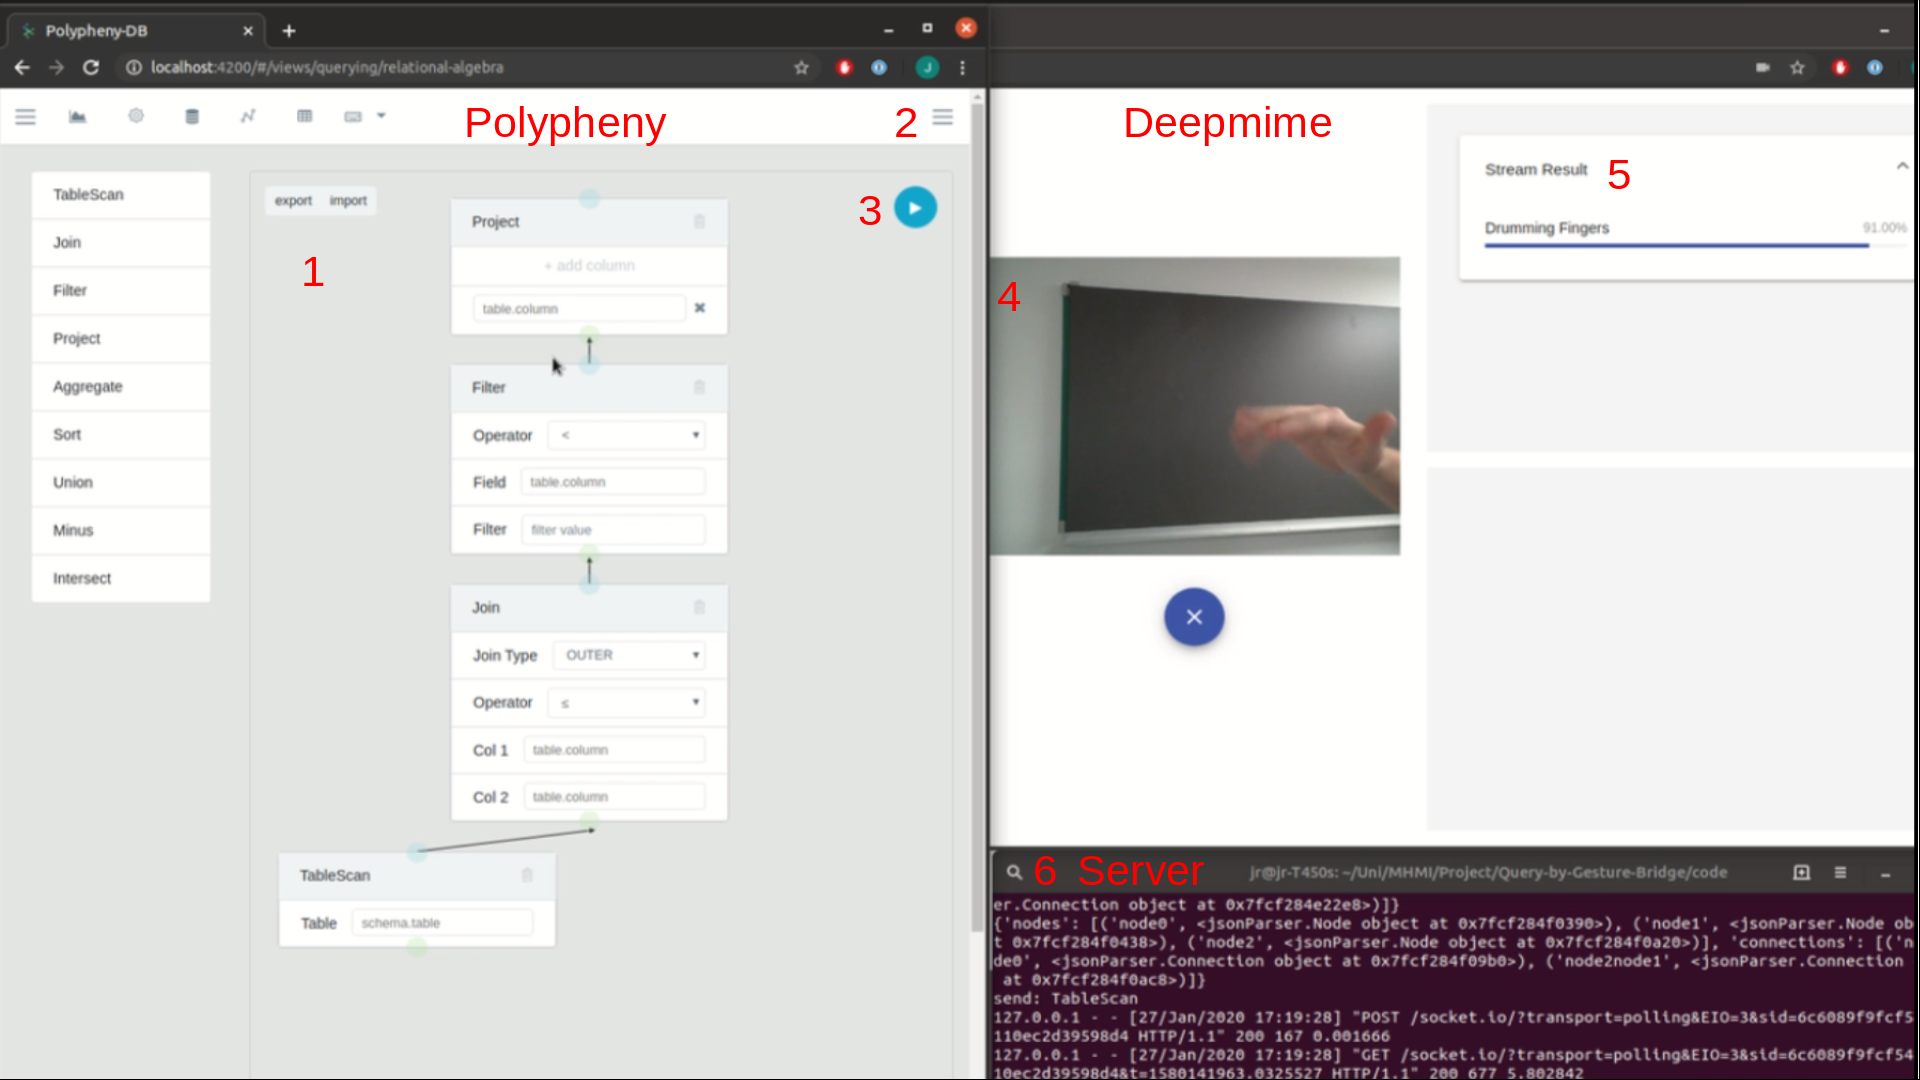
\includegraphics[width=\textwidth]{reportContent/images/example.png}
    \caption{Example layout of Query by Gesture}
    \label{fig:example}
    \begin{tabular}{r@{: }l r@{: }l}
    $1$& query plan builder & $4$ & video input \\
    $2$& settings & $5$ & found gesture with classification score\\
    $3$& run query  & $6$& terminal which runs the server 
    \end{tabular}
\end{figure}{}
\begin{figure}[H]
    \centering
    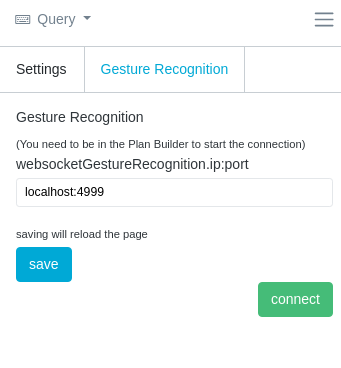
\includegraphics[width=0.6\textwidth]{reportContent/images/settings_s.png}
    \caption{Settings for Gesture Recognition in Polypheny}
    \label{fig:settings}
\end{figure}{}
\\
When everything is running and connected you can use the following  gestures to build a query:
\\
\\
\textbf{operators}
\begin{itemize}
    \item Drumming Fingers: TableScan
    \item Zooming In With Two Fingers: Join
    \item Zooming Out With Two Fingers: Join
    \item Pushing Hand Away: Project
    \item Pushing Hand In: Project
    \item Shaking Hand: Sort
    \item Stop Sign: Filter
\end{itemize}
\textbf{navigation}
\begin{itemize}
    \item Swiping Left: next
    \item Swiping Right: next
    \item Thumb Up: confirm
    \item Thumb Down: cancel
    \item Swiping Down: undo
    \item Swiping Up: undo
    \item Turning Hand Clockwise: delete
    \item Turning Hand Counterclockwise: 'delete
\end{itemize}
There are some things you need to know when building your query. The "Join" and "Filter" operators have two respectively one additional fields you have to specify via gesture control. You can do this via "next" (which goes through the possible options) and "confirm" (selects the shown option). Additionally the "undo" will delete the last inserted operator and the "delete" will get rid of the whole query.
\\
If you only want to insert queries without running it in the end it is enough if you run Polypheny-UI with \texttt{ng serve}. Furthermore you can mock Deepmime by simply running:
\begin{lstlisting}
python3 mock.py
\end{lstlisting}
In the terminal you can then type in the commands (e.g. TableScan, confirm, next etc.).  
\\
\\
Example videos:
\begin{itemize}
    \item Deepmime: \url{https://youtu.be/2SVj17GXv7s}
    \item Mock: \url{https://youtu.be/DYrqiwcTzNs}
\end{itemize}


